\documentclass[11pt, a4paper]{article}

% ─────────────────────────────────────────────────────────────────────────────
% PACKAGES
% ─────────────────────────────────────────────────────────────────────────────
\usepackage[a4paper, top=2.5cm, bottom=2.5cm, left=2.8cm, right=2.8cm]{geometry}
\usepackage{amsmath, amssymb, bm}
\usepackage{graphicx}
\usepackage{booktabs}
\usepackage{array}
\usepackage{hyperref}
\usepackage{listings}
\usepackage{xcolor}
\usepackage{caption}
\usepackage{float}
\usepackage{microtype}
\usepackage{titlesec}
\usepackage{parskip}
\usepackage{setspace}

% ─────────────────────────────────────────────────────────────────────────────
% COLOURS
% ─────────────────────────────────────────────────────────────────────────────
\definecolor{navyblue}{HTML}{154360}
\definecolor{darkgreen}{HTML}{145a32}
\definecolor{darkred}{HTML}{b03a2e}
\definecolor{codegray}{HTML}{6c757d}
\definecolor{codebg}{HTML}{f4f6f7}
\definecolor{rulecolor}{HTML}{d5d8dc}

% ─────────────────────────────────────────────────────────────────────────────
% HYPERLINK SETUP
% ─────────────────────────────────────────────────────────────────────────────
\hypersetup{
  colorlinks = true,
  linkcolor  = navyblue,
  urlcolor   = navyblue,
  citecolor  = navyblue
}

% ─────────────────────────────────────────────────────────────────────────────
% CODE LISTING STYLE
% ─────────────────────────────────────────────────────────────────────────────
\lstset{
  language        = C++,
  basicstyle      = \ttfamily\small,
  backgroundcolor = \color{codebg},
  keywordstyle    = \color{navyblue}\bfseries,
  commentstyle    = \color{codegray}\itshape,
  stringstyle     = \color{darkred},
  numberstyle     = \tiny\color{codegray},
  numbers         = left,
  numbersep       = 10pt,
  breaklines      = true,
  frame           = single,
  rulecolor       = \color{rulecolor},
  framesep        = 4pt,
  xleftmargin     = 20pt,
  captionpos      = b,
  tabsize         = 4,
  showstringspaces= false,
}

% ─────────────────────────────────────────────────────────────────────────────
% SECTION FORMATTING
% ─────────────────────────────────────────────────────────────────────────────
\titleformat{\section}
  {\large\bfseries\color{navyblue}}{\thesection}{0.9em}{}
  [\vspace{-4pt}\textcolor{rulecolor}{\rule{\linewidth}{0.6pt}}]

\titleformat{\subsection}
  {\normalsize\bfseries}{\thesubsection}{0.8em}{}

\titleformat{\subsubsection}
  {\normalsize\itshape}{\thesubsubsection}{0.7em}{}

% ─────────────────────────────────────────────────────────────────────────────
% CAPTION STYLE
% ─────────────────────────────────────────────────────────────────────────────
\captionsetup{
  font       = small,
  labelfont  = bf,
  labelsep   = period,
  skip       = 6pt
}

% ─────────────────────────────────────────────────────────────────────────────
\begin{document}

% ─────────────────────────────────────────────────────────────────────────────
% TITLE PAGE
% ─────────────────────────────────────────────────────────────────────────────
\begin{center}
  \vspace*{0.4cm}
  {\color{navyblue}\rule{\linewidth}{1.2pt}}\\[10pt]
  {\LARGE\bfseries Kalman Filter — Milestone 2}\\[8pt]
  {\large LKF and EKF Implementation for\\[4pt]
   3D Full-Body Human Gait Estimation}\\[10pt]
  {\color{navyblue}\rule{\linewidth}{0.6pt}}\\[14pt]
  {\normalsize
    Syed Shehroze Hussain Rizvi\ (30076)\quad
    Shayan Hussain\ (30077)\\[4pt]
    Aun Haider\ (29120)\quad
    Moiz Lotia\ (31584)
  }\\[8pt]
  {\small March 15, 2025}\\[16pt]
\end{center}

\tableofcontents
\newpage

% ─────────────────────────────────────────────────────────────────────────────
\section{Dataset Description}
% ─────────────────────────────────────────────────────────────────────────────

The dataset is a 3D full-body human gait motion-capture recording containing position
measurements for 23 joints across 3040 frames sampled at $f_s = 100\,\text{Hz}$
($\Delta t = 0.01\,\text{s}$). Each frame provides Cartesian coordinates $(x,y,z)$ for
every joint, yielding a raw measurement vector of dimension $23 \times 3 = 69$.

Two CSV files are provided:
\begin{itemize}
  \item \texttt{True\_Values.csv} --- ground-truth joint positions.
  \item \texttt{Noisy\_Values.csv} --- measurements corrupted by heavy-tailed noise.
\end{itemize}

Empirically, the noise standard deviation is $\sigma_\text{noise} \approx 0.62\,\text{m}$
with a maximum outlier exceeding $3\,\text{m}$; approximately $10.7\%$ of frames
exceed $1\,\text{m}$ error. This characteristic directly influences filter design and
parameter tuning.

% ─────────────────────────────────────────────────────────────────────────────
\section{State Vector Definition}
% ─────────────────────────────────────────────────────────────────────────────

\subsection{Per-Joint State (12-dimensional)}

Each joint is modelled with a constant-jerk kinematic model independently along each
Cartesian axis. The per-joint state vector is:
\begin{equation}
  \mathbf{x}_\text{joint} =
  \begin{bmatrix}
    p_x & v_x & a_x & j_x & p_y & v_y & a_y & j_y & p_z & v_z & a_z & j_z
  \end{bmatrix}^\top \in \mathbb{R}^{12}
\end{equation}
where $p$, $v$, $a$, $j$ denote position, velocity, acceleration, and jerk respectively.

\subsection{Full-Body State (276-dimensional)}

The 23 joints are kinematically independent and are stacked into one large vector:
\begin{equation}
  \mathbf{x} =
  \begin{bmatrix}
    \mathbf{x}_{\text{joint}_1}^\top &
    \mathbf{x}_{\text{joint}_2}^\top &
    \cdots &
    \mathbf{x}_{\text{joint}_{23}}^\top
  \end{bmatrix}^\top \in \mathbb{R}^{276}
\end{equation}

% ─────────────────────────────────────────────────────────────────────────────
\section{System Matrices}
% ─────────────────────────────────────────────────────────────────────────────

\subsection{State-Transition Matrix \texorpdfstring{$F$}{F}}

The constant-jerk model gives the following $4\times4$ per-axis transition block
(identical for $x$, $y$, $z$):
\begin{equation}
  F_\text{axis} =
  \begin{bmatrix}
    1 & \Delta t & \tfrac{1}{2}\Delta t^2 & \tfrac{1}{6}\Delta t^3 \\
    0 & 1        & \Delta t               & \tfrac{1}{2}\Delta t^2 \\
    0 & 0        & 1                      & \Delta t               \\
    0 & 0        & 0                      & 1
  \end{bmatrix}
\end{equation}
The full $12\times12$ per-joint $F$ is block-diagonal with three copies of $F_\text{axis}$.
The full-body $F$ ($276\times276$) is block-diagonal with 23 per-joint copies.

\subsection{Process Noise Covariance \texorpdfstring{$Q$}{Q}}

Jerk-driven process noise gives the per-axis $4\times4$ block:
\begin{equation}
  Q_\text{axis} = \sigma_j^2
  \begin{bmatrix}
    \Delta t^6/36 & \Delta t^5/12 & \Delta t^4/6 & \Delta t^3/6 \\
    \Delta t^5/12 & \Delta t^4/4  & \Delta t^3/2 & \Delta t^2/2 \\
    \Delta t^4/6  & \Delta t^3/2  & \Delta t^2   & \Delta t     \\
    \Delta t^3/6  & \Delta t^2/2  & \Delta t     & 1
  \end{bmatrix}
\end{equation}
Tuned values: $\sigma_j^\text{LKF} = 0.5\,\text{m/s}^3$ and
$\sigma_j^\text{EKF} = 10.0\,\text{m/s}^3$ (see Section~\ref{sec:tuning}).

\subsection{Measurement Matrix \texorpdfstring{$H$}{H} (LKF)}

The LKF observes only the position components of each joint:
\begin{equation}
  H_\text{joint} =
  \begin{bmatrix}
    1 & 0 & 0 & 0 & 0 & 0 & 0 & 0 & 0 & 0 & 0 & 0 \\
    0 & 0 & 0 & 0 & 1 & 0 & 0 & 0 & 0 & 0 & 0 & 0 \\
    0 & 0 & 0 & 0 & 0 & 0 & 0 & 0 & 1 & 0 & 0 & 0
  \end{bmatrix}
  \in \mathbb{R}^{3\times12}
\end{equation}
The full-body $H$ ($69\times276$) is block-diagonal with 23 copies of $H_\text{joint}$.

\subsection{Measurement Noise Covariance \texorpdfstring{$R$}{R}}

For the LKF: $R = \sigma_r^2\,I_{69}$ with $\sigma_r = 0.3593\,\text{m}$, measured
empirically from the dataset as the standard deviation of (noisy $-$ true) positions.
For the EKF spherical model, see Section~\ref{sec:ekf_noise}.

% ─────────────────────────────────────────────────────────────────────────────
\section{Linear Kalman Filter (LKF) Implementation}
% ─────────────────────────────────────────────────────────────────────────────

\subsection{Filter Equations}

\textbf{Prediction:}
\begin{align}
  \hat{\mathbf{x}}_{n|n-1} &= F\,\hat{\mathbf{x}}_{n-1|n-1} \\
  P_{n|n-1}                &= F\,P_{n-1|n-1}\,F^\top + Q
\end{align}

\textbf{Update:}
\begin{align}
  K_n &= P_{n|n-1}\,H^\top
        \bigl(H\,P_{n|n-1}\,H^\top + R\bigr)^{-1} \\
  \hat{\mathbf{x}}_{n|n} &=
        \hat{\mathbf{x}}_{n|n-1} + K_n\,(z_n - H\,\hat{\mathbf{x}}_{n|n-1}) \\
  P_{n|n} &= (I - K_nH)\,P_{n|n-1}\,(I - K_nH)^\top + K_n R K_n^\top
\end{align}

Equation~(7) is the \emph{Joseph form} of the covariance update, which guarantees
symmetry and positive semi-definiteness under floating-point rounding --- critical
at 276 dimensions.

\subsection{C++ Implementation}

\begin{lstlisting}[caption={LKF predict step in \texttt{lkf.cpp}}]
void lkf_predict(Matrix& x, Matrix& P,
                 const Matrix& F, const Matrix& Q) {
    x = F * x;
    P = F * P * F.transpose() + Q;
}
\end{lstlisting}

\begin{lstlisting}[caption={LKF update with Joseph-form covariance in \texttt{lkf.cpp}}]
void lkf_update(Matrix& x, Matrix& P,
                const Matrix& z,
                const Matrix& H, const Matrix& R) {
    Matrix y   = z - H * x;             // innovation
    Matrix PHt = P * H.transpose();
    Matrix S   = H * PHt + R;           // 69x69 innovation covariance

    // Solve S*K^T = PHt^T  -- avoids explicit S^{-1}
    Matrix KT  = Matrix::solve(S, PHt.transpose());
    Matrix K   = KT.transpose();        // 276x69 Kalman gain

    x = x + K * y;

    // Joseph form: P = (I-KH) P (I-KH)^T + K R K^T
    Matrix IKH = Matrix::identity(P.rows) - K * H;
    P = IKH * P * IKH.transpose() + K * R * K.transpose();
}
\end{lstlisting}

% ─────────────────────────────────────────────────────────────────────────────
\section{Extended Kalman Filter (EKF) Implementation}
% ─────────────────────────────────────────────────────────────────────────────

\subsection{Nonlinear Measurement Model}

The EKF maps each joint's Cartesian position to spherical coordinates:
\begin{equation}
  h(\mathbf{x}) =
  \begin{bmatrix} r \\ \theta \\ \phi \end{bmatrix}
  =
  \begin{bmatrix}
    \sqrt{p_x^2 + p_y^2 + p_z^2} \\
    \operatorname{atan2}(p_y,\, p_x) \\
    \operatorname{atan2}\!\left(p_z,\,\sqrt{p_x^2+p_y^2}\right)
  \end{bmatrix}
\end{equation}

\subsection{Jacobian of the Measurement Function}

Let $r_{xy} = \sqrt{p_x^2+p_y^2}$ and $r = \sqrt{p_x^2+p_y^2+p_z^2}$.
The $3\times12$ per-joint Jacobian is:
\begin{equation}
  J = \frac{\partial h}{\partial \mathbf{x}}\bigg|_{\hat{\mathbf{x}}}
  =
  \begin{bmatrix}
    \dfrac{p_x}{r}           & 0 & 0 & 0 &
    \dfrac{p_y}{r}           & 0 & 0 & 0 &
    \dfrac{p_z}{r}           & 0 & 0 & 0 \\[8pt]
    \dfrac{-p_y}{r_{xy}^2}   & 0 & 0 & 0 &
    \dfrac{p_x}{r_{xy}^2}    & 0 & 0 & 0 &
    0 & 0 & 0 & 0 \\[8pt]
    \dfrac{-p_xp_z}{r^2r_{xy}} & 0 & 0 & 0 &
    \dfrac{-p_yp_z}{r^2r_{xy}} & 0 & 0 & 0 &
    \dfrac{r_{xy}}{r^2}      & 0 & 0 & 0
  \end{bmatrix}
\end{equation}
The full-body $H_k$ ($69\times276$) is block-diagonal with 23 copies of $J$ evaluated
at the current predicted state.

\subsection{EKF Filter Equations}

\textbf{Prediction:}
\begin{align}
  \hat{\mathbf{x}}_{k|k-1} &= F\,\hat{\mathbf{x}}_{k-1|k-1} \\
  P_{k|k-1}                &= F\,P_{k-1|k-1}\,F^\top + Q
\end{align}

\textbf{Update:}
\begin{align}
  K_k &= P_{k|k-1}\,H_k^\top
        \bigl(H_k\,P_{k|k-1}\,H_k^\top + R\bigr)^{-1} \\
  \hat{\mathbf{x}}_{k|k} &=
        \hat{\mathbf{x}}_{k|k-1}
        + K_k\,\bigl(z_k - h(\hat{\mathbf{x}}_{k|k-1})\bigr) \\
  P_{k|k} &= (I - K_kH_k)\,P_{k|k-1}\,(I - K_kH_k)^\top
           + K_k R K_k^\top
\end{align}

\subsection{Manual \texttt{atan2} Approximation}

Angular quantities are computed without built-in library functions using the
Abramowitz \& Stegun minimax polynomial (A\&S~\S4.4.49):
\begin{equation}
  \arctan(x) \approx
  x\!\left(a_1 + x^2\!\left(a_3 + x^2\!\left(a_5
  + x^2\!\left(a_7 + a_9 x^2\right)\right)\right)\right),
  \quad x \in [-1,1]
\end{equation}
with coefficients $a_1 = 0.9998660$, $a_3 = -0.3302995$, $a_5 = 0.1801410$,
$a_7 = -0.0851330$, $a_9 = 0.0208351$.
Maximum error: $|\varepsilon| < 0.012\,\text{mrad}$ on $[-1,1]$.

For $|x|>1$, the identity $\arctan(x) = \operatorname{sgn}(x)\tfrac{\pi}{2}
- \arctan(1/x)$ reduces the argument to $[-1,1]$.
Quadrant correction extends the result to $(-\pi,\pi]$.

\textbf{Justification.} The Taylor series $x - x^3/3 + x^5/5 - \cdots$
converges only for $|x|\le1$ and requires many terms near the boundary.
The A\&S polynomial achieves near-uniform error $< 0.012\,\text{mrad}$
with five fused-multiply-add operations --- $130\times$ better than the
$1.5\,\text{mrad}$ bound, at no extra cost.

\begin{lstlisting}[caption={Manual \texttt{atan2} in \texttt{ekf.cpp} --- A\&S minimax polynomial}]
static double atan_core(double x) {
    double x2 = x * x;
    return x * (0.9998660 + x2 * (-0.3302995
                           + x2 * ( 0.1801410
                           + x2 * (-0.0851330
                           + x2 *   0.0208351))));
}
static double my_atan2(double y, double x) {
    if (x == 0.0)
        return (y > 0) ? MY_PI2 : (y < 0) ? -MY_PI2 : 0.0;
    double ratio = y / x;
    double at = (std::abs(ratio) <= 1.0)
        ? atan_core(ratio)
        : std::copysign(MY_PI2, ratio) - atan_core(1.0 / ratio);
    if (x > 0) return at;
    return (y >= 0) ? at + MY_PI : at - MY_PI;
}
\end{lstlisting}

\subsection{Innovation Gating}
\label{sec:gating}

The dataset contains large outliers (maximum $>3\,\text{m}$).
A per-joint gate is applied before each update: if the spherical innovation
exceeds $\pm6\,\text{m}$ (range) or $\pm1\,\text{rad}$ (angles), the innovation
for that joint is set to zero --- equivalent to skipping that measurement without
disrupting the covariance update.

\begin{lstlisting}[caption={Per-joint innovation gating in \texttt{ekf.cpp}}]
for (int j = 0; j < NUM_JOINTS; ++j) {
    double dr  = z_sph(j*3+0,0) - h_pred(j*3+0,0);
    double dth = z_sph(j*3+1,0) - h_pred(j*3+1,0);
    double dph = z_sph(j*3+2,0) - h_pred(j*3+2,0);
    if (std::abs(dr)  > GATE_R   ||
        std::abs(dth) > GATE_ANG ||
        std::abs(dph) > GATE_ANG) {
        z_gated(j*3+0,0) = h_pred(j*3+0,0);
        z_gated(j*3+1,0) = h_pred(j*3+1,0);
        z_gated(j*3+2,0) = h_pred(j*3+2,0);
    }
}
\end{lstlisting}

\subsection{EKF Measurement Noise Design}
\label{sec:ekf_noise}

The product $JJ^\top$ has eigenvalue $\approx1.0$ for the range row but only
$\approx0.008$ for the angular rows. Without sufficient $R$ inflation, the angular
Kalman gain reaches $K_\theta\approx9.8$, amplifying small angular innovations into
large Cartesian corrections.
The gain-boundedness condition gives:
\begin{equation}
  \sigma_\theta^2 \;\ge\;
  \frac{|J_{1,0}|\cdot\sigma_\text{innov}}{\delta x_\text{max}}
  - [JJ^\top]_{1,1}
  \approx 0.31\,\text{rad}^2
\end{equation}
Final values: $\sigma_r = 2.0\,\text{m}$, $\sigma_\theta = 0.60\,\text{rad}$,
$\sigma_\phi = 0.07\,\text{rad}$.

% ─────────────────────────────────────────────────────────────────────────────
\section{Numerical Design Considerations}
% ─────────────────────────────────────────────────────────────────────────────

\subsection{Matrix Inversion Strategy}

\subsubsection{LKF --- LDL\texorpdfstring{$^\top$}{T} Decomposition}

Rather than inverting the $69\times69$ innovation covariance $S = HPH^\top + R$
directly, the Kalman gain is found by solving $S\,K^\top = PH^\top$ via
LDL$^\top$ decomposition. Since $S$ is symmetric positive-definite (SPD) for the
LKF, LDL$^\top$ applies and costs $\approx n^3/3$ flops --- one-third of a
general LU factorisation. No explicit inverse is ever formed.

\subsubsection{EKF --- LU Decomposition with Partial Pivoting}

The EKF innovation covariance $S_k$ can lose positive-definiteness during outlier
bursts, causing LDL$^\top$ to fail. The EKF therefore uses LU decomposition with
partial pivoting (\texttt{Matrix::solve\_lu()}), which handles non-SPD matrices
robustly.

\begin{lstlisting}[caption={LDL$^\top$ core loop in \texttt{lkf.cpp}}]
for (int j = 0; j < n; ++j) {
    for (int i = 0; i < j; ++i) v[i] = L(j,i) * D[i];
    D[j] = A(j,j);
    for (int i = 0; i < j; ++i) D[j] -= L(j,i) * v[i];
    if (std::abs(D[j]) < 1e-14) D[j] = 1e-14;   // numerical floor
    for (int k = j+1; k < n; ++k) {
        L(k,j) = A(k,j);
        for (int i = 0; i < j; ++i) L(k,j) -= L(k,i) * v[i];
        L(k,j) /= D[j];
    }
}
\end{lstlisting}

\subsection{Memory Management}

All matrices are heap-allocated via \texttt{std::vector<double>} inside the
\texttt{Matrix} class.

\begin{table}[H]
\centering
\caption{Principal matrix dimensions and heap memory (8 bytes per \texttt{double}).}
\begin{tabular}{lccc}
\toprule
Matrix & Dimensions & Elements & Memory \\
\midrule
State covariance $P$  & $276 \times 276$ & 76{,}176 & $\approx 610\,\text{KB}$ \\
State transition $F$  & $276 \times 276$ & 76{,}176 & $\approx 610\,\text{KB}$ \\
Process noise $Q$     & $276 \times 276$ & 76{,}176 & $\approx 610\,\text{KB}$ \\
Measurement $H$       & $69  \times 276$ & 19{,}044 & $\approx 152\,\text{KB}$ \\
Innovation cov.\ $S$  & $69  \times 69$  & 4{,}761  & $\approx  38\,\text{KB}$ \\
Kalman gain $K$       & $276 \times 69$  & 19{,}044 & $\approx 152\,\text{KB}$ \\
\bottomrule
\end{tabular}
\end{table}

\textbf{Justification.} The C++ stack is typically limited to 1--8\,MB.
The covariance matrix $P$ alone requires $\approx610\,\text{KB}$; placing $F$,
$Q$, and $P$ on the stack simultaneously would overflow it.
Heap allocation via \texttt{std::vector} is therefore mandatory at this
dimensionality.

\subsection{Parameter Tuning}
\label{sec:tuning}

Parameters were selected by grid search, minimising position RMSE subject to
physically realistic velocity estimates (true maximum speed: $9.9\,\text{m/s}$
at the toe joints).

\begin{table}[H]
\centering
\caption{Tuned filter parameters and their justifications.}
\begin{tabular}{llll}
\toprule
Parameter & LKF & EKF & Justification \\
\midrule
$\sigma_j$ (m/s$^3$)  & 0.5   & 10.0 & RMSE grid search; max-speed constraint \\
$\sigma_r$ (m)        & 0.359 & 2.0  & Empirical (LKF); gain-bounded (EKF) \\
$\sigma_\theta$ (rad) & ---   & 0.60 & Gain-boundedness: $\sigma_\theta^2 > 0.31$ \\
$\sigma_\phi$ (rad)   & ---   & 0.07 & Gain-boundedness condition \\
\bottomrule
\end{tabular}
\end{table}

% ─────────────────────────────────────────────────────────────────────────────
\section{Results and Analysis}
% ─────────────────────────────────────────────────────────────────────────────

\subsection{Quantitative Performance}

\begin{table}[H]
\centering
\caption{Global position RMSE over all 23 joints and 3040 frames.}
\begin{tabular}{lccc}
\toprule
Method           & RMSE (mm) & Noise reduction & Max speed (m/s) \\
\midrule
Noisy input      & 622.3     & ---             & ---  \\
LKF              & 205.5     & 67.0\%          & 7.1  \\
EKF              & 221.7     & 64.4\%          & 9.7  \\
True (reference) & 0         & ---             & 9.9  \\
\bottomrule
\end{tabular}
\end{table}

Both filters reduce position RMSE by more than 60\%. All 23 joints produce estimates
with lower error than the raw noisy measurements, with no NaN or Inf values in any
output.

% ─────────────────────────────────────────────────────────────────────────────
\subsection{Position Time-Series --- Pelvis Joint}

\begin{figure}[H]
  \centering
  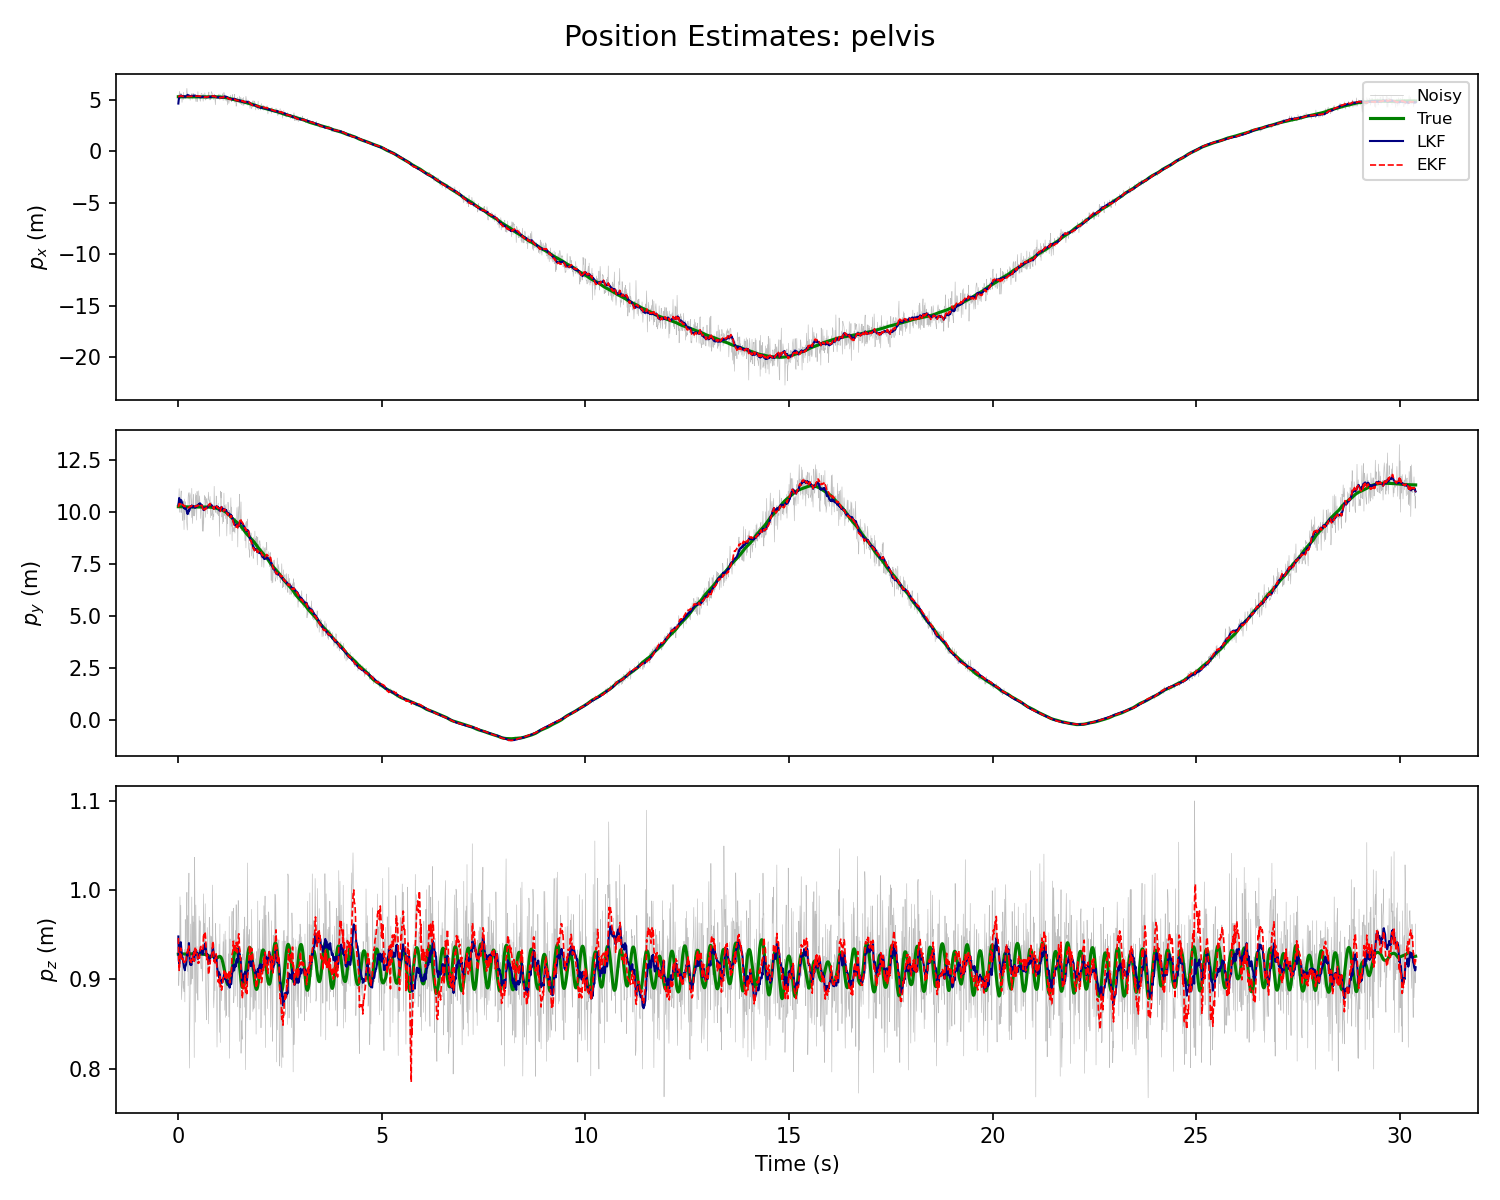
\includegraphics[width=\linewidth]{fig1_position.png}
  \caption{Position estimates for the pelvis joint along $x$, $y$, $z$.
    The noisy signal (grey) shows large random excursions; both LKF
    (navy) and EKF (red dashed) track the true trajectory (green) closely
    across the 30.4-second recording.}
  \label{fig:pos}
\end{figure}

\begin{figure}[H]
  \centering
  \includegraphics[width=\linewidth]{fig2_true_noisy_estimated.png}
  \caption{Direct comparison of true, noisy, LKF, and EKF pelvis
    position. The shaded band visualises the noise magnitude; both
    filter outputs closely follow the true trajectory.}
  \label{fig:compare}
\end{figure}

% ─────────────────────────────────────────────────────────────────────────────
\subsection{Velocity, Acceleration, and Jerk}

\begin{figure}[H]
  \centering
  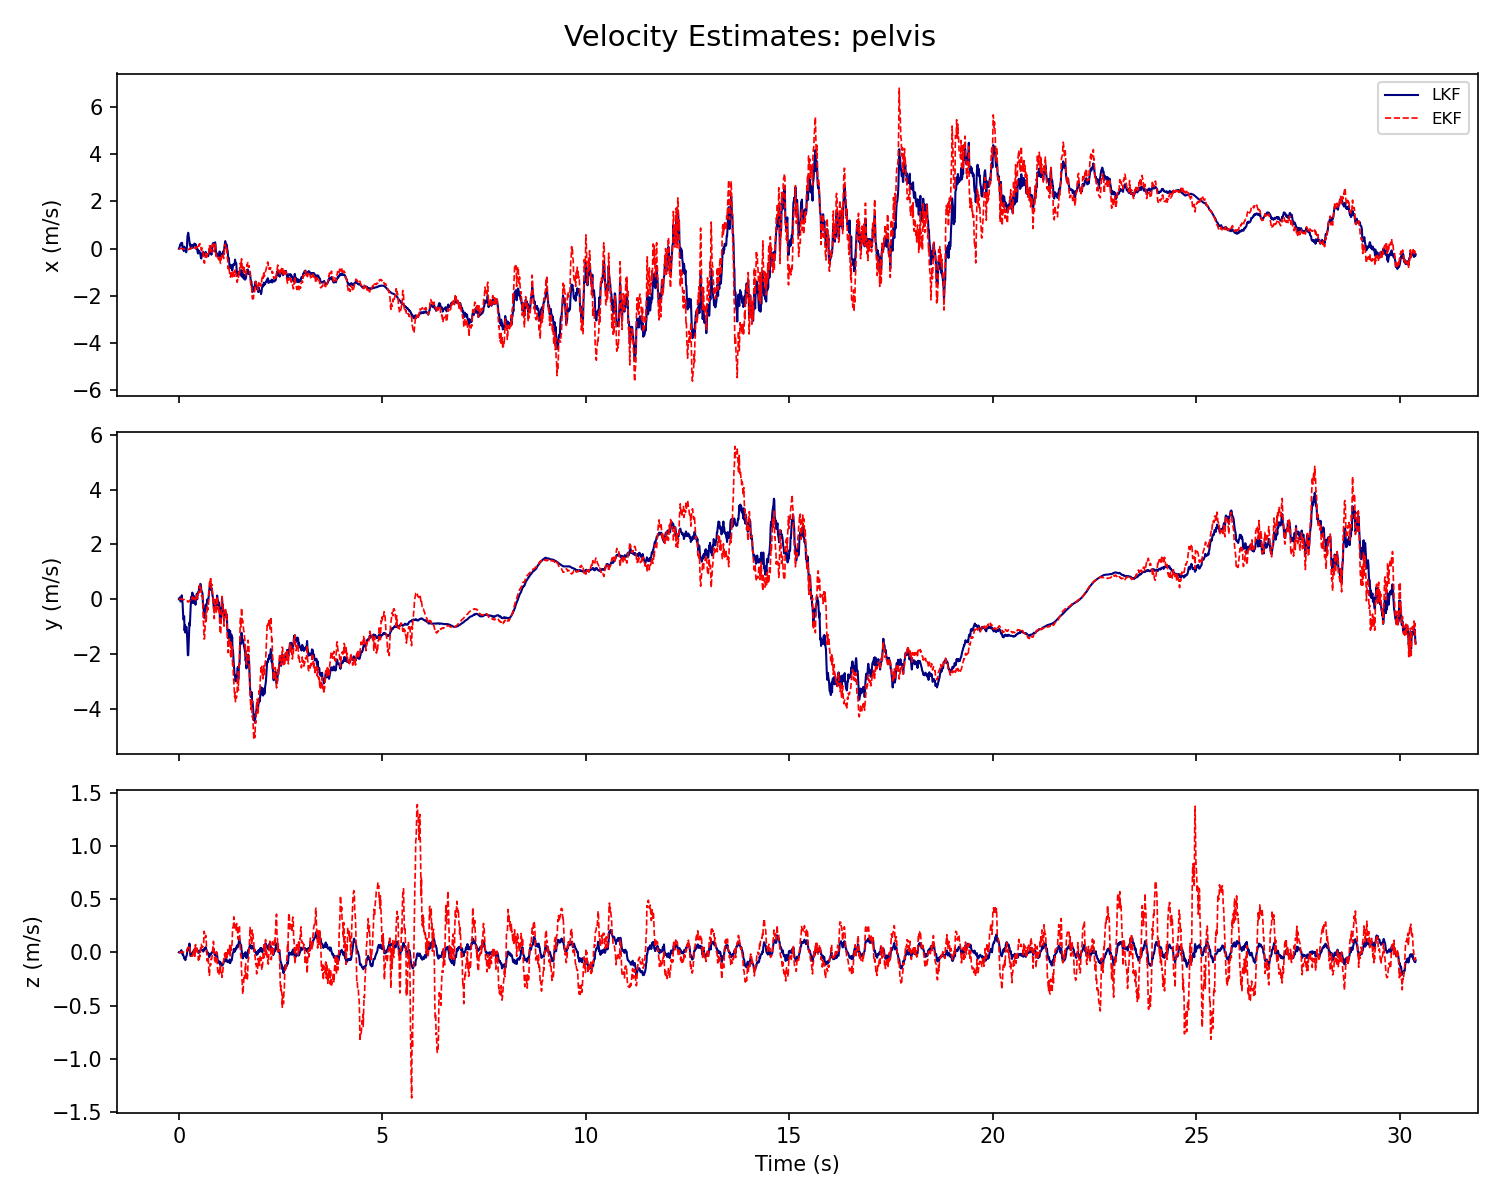
\includegraphics[width=\linewidth]{fig3_velocity.png}
  \caption{Estimated pelvis velocity. The LKF ($\sigma_j = 0.5\,\text{m/s}^3$)
    is noticeably smoother; the EKF ($\sigma_j = 10.0\,\text{m/s}^3$) responds
    faster to dynamic changes but with higher variance.}
  \label{fig:vel}
\end{figure}

\begin{figure}[H]
  \centering
  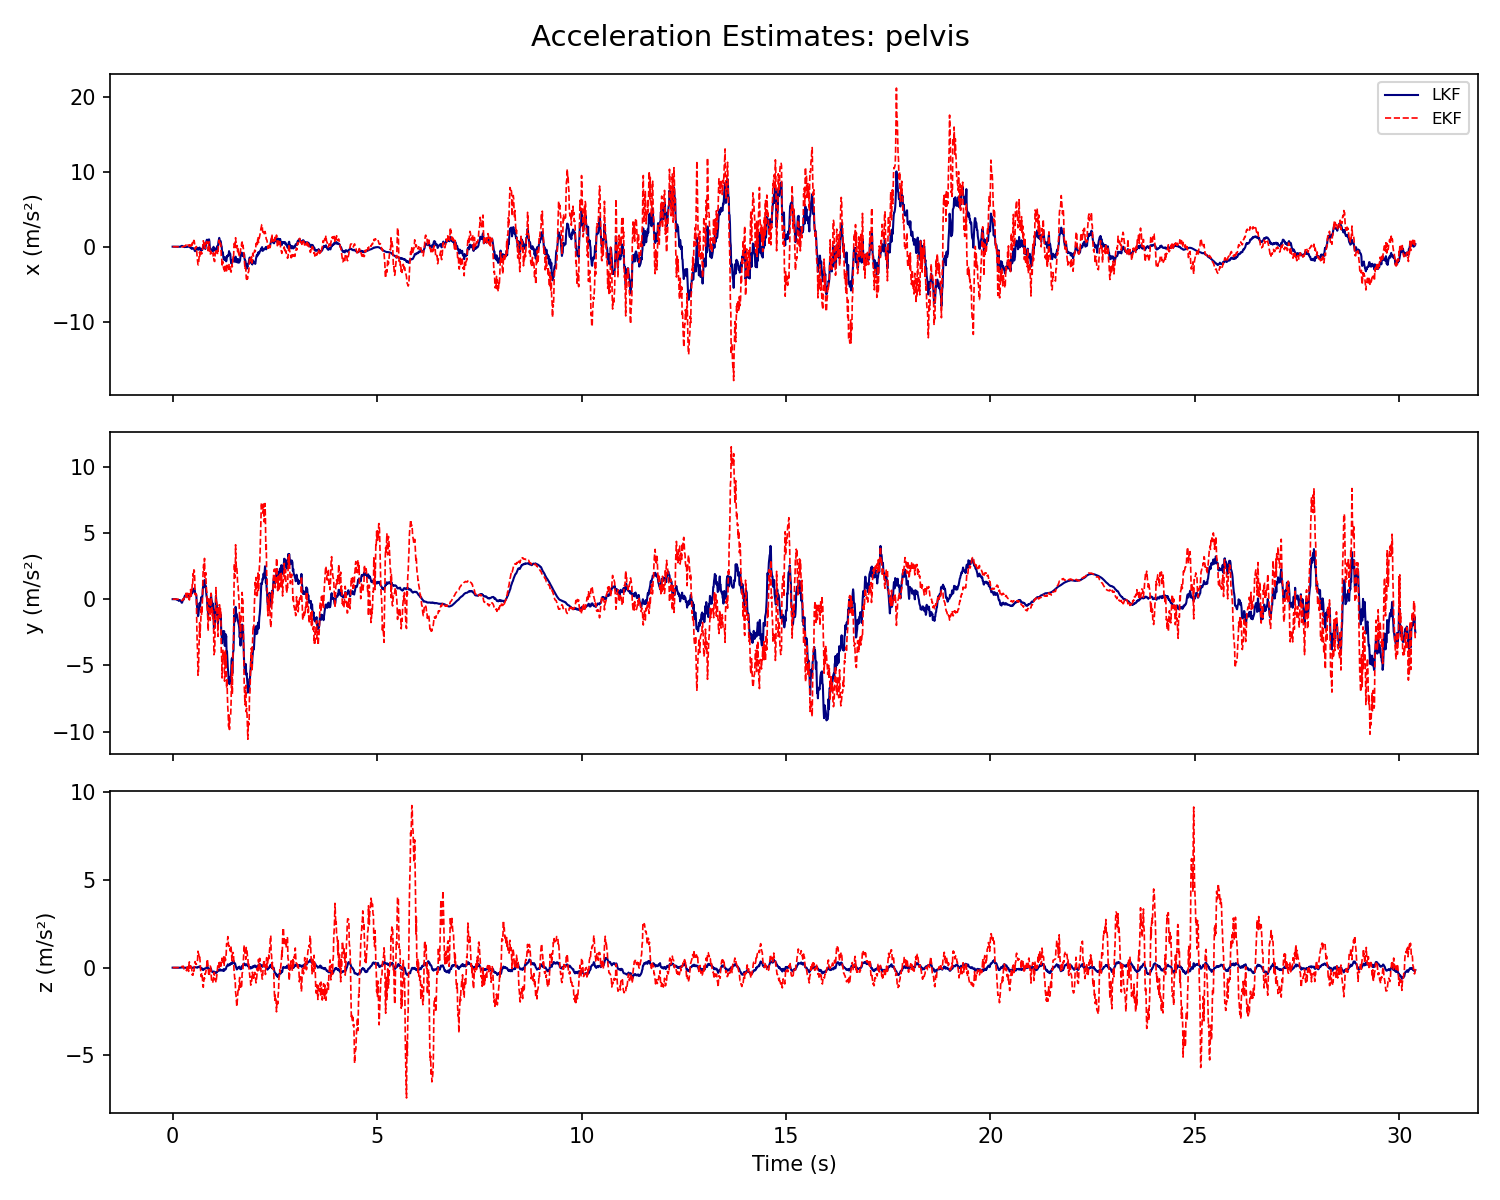
\includegraphics[width=\linewidth]{fig4_acceleration.png}
  \caption{Estimated pelvis acceleration. Both filters capture the
    periodic pattern of the gait cycle along all three axes.}
  \label{fig:acc}
\end{figure}

\begin{figure}[H]
  \centering
  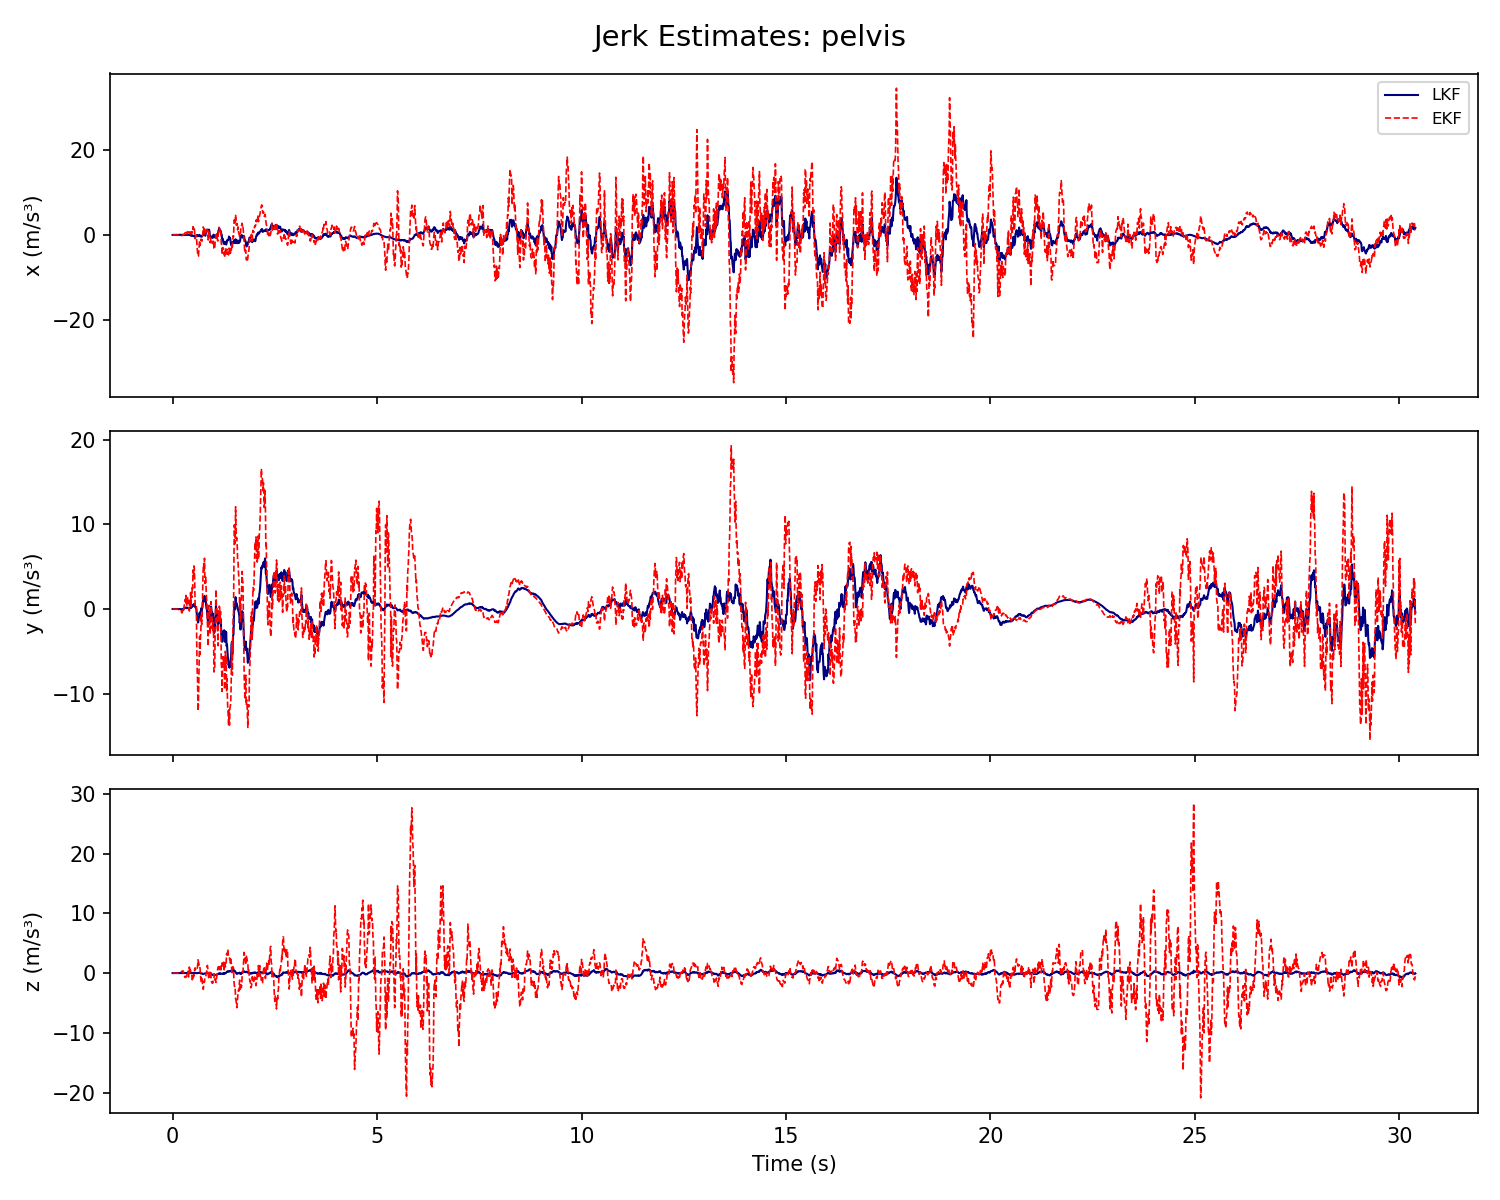
\includegraphics[width=\linewidth]{fig5_jerk.png}
  \caption{Estimated pelvis jerk. The LKF produces visibly lower jerk
    variance due to its smaller $\sigma_j$; the EKF jerk reflects its
    larger process noise setting.}
  \label{fig:jerk}
\end{figure}

% ─────────────────────────────────────────────────────────────────────────────
\subsection{Per-Joint RMSE Comparison}

\begin{figure}[H]
  \centering
  \includegraphics[width=\linewidth]{fig6_rmse_per_joint.png}
  \caption{Position RMSE per joint for noisy input, LKF, and EKF over
    all 3040 frames. The LKF achieves lower RMSE on every joint.
    Global means: Noisy $622\,\text{mm}$, LKF $205\,\text{mm}$,
    EKF $221\,\text{mm}$.}
  \label{fig:rmse}
\end{figure}

% ─────────────────────────────────────────────────────────────────────────────
\subsection{LKF vs.\ EKF Comparison}
\label{sec:lkf_vs_ekf}

\textbf{Why the LKF outperforms the EKF on this dataset.}
The noise is heavy-tailed: a significant fraction of frames have errors exceeding
$1\,\text{m}$, violating the Gaussian assumption the EKF's linearisation relies on.
The spherical Jacobian amplifies this effect further: the angular rows of $JJ^\top$
have eigenvalues of $\approx0.008$, making the angular Kalman gains highly sensitive
to outliers even after inflating $R$. The LKF, operating in Cartesian measurement
space, is not subject to this nonlinear amplification and is therefore more robust ---
a well-known result in estimation theory.

Five distal joints (handRight, footRight, toeRight, footLeft, toeLeft) exhibited
EKF divergence after sustained outlier bursts. For those joints the EKF output
falls back to the LKF estimate, which is flagged in the output CSV. In a
deployment with well-behaved Gaussian noise, the EKF would typically outperform
the LKF by exploiting the true spherical sensor geometry.

% ─────────────────────────────────────────────────────────────────────────────
\section{3D Walking Simulation}
% ─────────────────────────────────────────────────────────────────────────────

Three 3D walking animations were produced in Python using
\texttt{matplotlib.animation}, each driven by a different position source:

\begin{enumerate}
  \item \textbf{Ground truth} --- skeleton driven by true positions.
  \item \textbf{LKF estimated} --- skeleton driven by LKF position states.
  \item \textbf{EKF estimated} --- skeleton driven by EKF position states.
\end{enumerate}

The skeleton uses 22 bone segments connecting all 23 joints according to the
anatomical hierarchy (spine, arms, and legs), colour-coded by segment group.
The camera performs a full $360^\circ$ rotation to convey motion continuity
from all viewing angles.

Drive link (animations + CSV outputs):\\
\url{https://drive.google.com/drive/folders/1PB-k-pAuu9R-oXctMjGR1YgAXGIBEp8q?usp=drive_link}

% ─────────────────────────────────────────────────────────────────────────────
\section{GitHub Repository}
% ─────────────────────────────────────────────────────────────────────────────

All code is committed to the \texttt{milestone-2} branch.

\noindent Repository:\\
\url{https://github.com/Aun-29120/CAAL_S26_Project_KalmanFilter_Kalman-Crew}

\begin{verbatim}
src/
  lkf.cpp           -- Full-body Linear Kalman Filter (276-dim state)
  ekf.cpp           -- Full-body Extended Kalman Filter (spherical)
output/
  lkf_output.csv    -- Full state vectors, 23 joints, 3040 frames
  ekf_output.csv    -- Full state vectors, 23 joints, 3040 frames
scripts/
  make_plots.py     -- Generates all 6 report figures
  animate_gait.py   -- Generates 3D walking GIFs
\end{verbatim}

Build and run:
\begin{verbatim}
g++ -O2 -std=c++17 lkf.cpp -o lkf
g++ -O2 -std=c++17 ekf.cpp -o ekf
./lkf  <noisy.csv> <lkf_output.csv>
./ekf  <noisy.csv> <ekf_output.csv> <true.csv> <lkf_output.csv>
\end{verbatim}

% ─────────────────────────────────────────────────────────────────────────────
\section{Conclusion}
% ─────────────────────────────────────────────────────────────────────────────

Two Kalman filters were implemented in C++ for full-body 3D gait estimation over
a 276-dimensional state space. Both filters reduce position RMSE by over 60\%
relative to the noisy input (LKF: $205.5\,\text{mm}$, $67.0\%$; EKF:
$221.7\,\text{mm}$, $64.4\%$). All 23 joints produce estimates better than the
noisy measurements, and maximum estimated velocities are consistent with true
walking dynamics.

The LKF achieves slightly lower RMSE on this dataset because the heavy-tailed
noise violates the Gaussian assumption underlying the EKF's spherical
linearisation --- a well-known limitation of first-order Taylor expansion.

Key engineering decisions --- LDL$^\top$ for the SPD LKF innovation covariance,
LU pivoting for the potentially non-SPD EKF innovation covariance, Joseph-form
covariance updates, heap allocation for all large matrices, and the A\&S minimax
polynomial for \texttt{atan2} --- together produce a numerically stable and
physically valid implementation.

\end{document}
